\documentclass[11pt,letterpaper,twocolumn]{fenbil}

% İki sütun arasında taşma sorununu engellemek için paketler
\usepackage{amsmath,amssymb,amsfonts}
\usepackage{graphicx}
\usepackage{tcolorbox}
\usepackage{tikz}
\usepackage{physics}
\usepackage{microtype} % Taşma sorunlarını azaltmak için
\usepackage{geometry}
\geometry{margin=2.5cm} % Sayfa kenar boşluklarını ayarla
\usepackage{ragged2e} % Daha iyi hizalama
\usepackage{cuted} % strip ortamı için
\usepackage{breqn} % otomatik denklem kırılımı için
\usepackage{mathtools} % Gelişmiş matematik araçları
\usepackage{circuitikz} % Elektrik devre çizimleri için

% Satır arası boşlukları azalt
\setlength{\abovedisplayskip}{3pt}
\setlength{\belowdisplayskip}{3pt}
\setlength{\abovedisplayshortskip}{3pt}
\setlength{\belowdisplayshortskip}{3pt}

% Sütun yapısını düzenle
\setlength{\columnsep}{15pt} % Sütunlar arası boşluğu azalt

\begin{document}
\twocolumn[
\begin{@twocolumnfalse}
\begin{minipage}{0.15\textwidth}
{
\includegraphics[width=4cm]{logo/iufizik.png}
}
\end{minipage}
\hspace{25pt}
\begin{minipage}{0.75\textwidth}
\vspace{5mm}
\Large{\textbf{ELEKTRONİK I - ANALOG ELEKTRONİK \\ 18 MART 2025}}
\vspace{3mm}\\
\large{\textbf{Ad Soyad:} Celal Ekrem Torun - 0411230037}
\vspace{2mm}\\
\large{\textbf{DERS:} Doç. Dr. Neslihan Üzar Kılıç}\newline
\fontsize{0.35cm}{0.5cm}\selectfont
\textit{Fizik Bölümü, İstanbul Üniversitesi\newline
Beyazıt, Fatih, İstanbul, Türkiye\newline
18 MART 2025}
\end{minipage}
\small
\end{@twocolumnfalse}]

% Dosya adını belgenin en üstünde göster
\begin{center}
\textbf{Dosya Adı:} FZKT2404\_ElektronikI\_H05S1\_RCveRLDevreleri.tex
\end{center}

\section{RC ve RL Devrelerinde Geçici Rejim Analizi}

Bu bölümde, kapasitör ve indüktör içeren devrelerde anahtar açılıp kapatıldığında oluşan geçici rejim davranışlarını inceleyeceğiz. Bu tür devrelerde enerjinin depolanması ve boşaltılması, zamanla değişen bir karakteristiğe sahiptir.

\subsection{Zaman Sabiti Kavramı}

\begin{tcolorbox}[title=ÖNEMLİ]
Enerji depo edebilen elemanlarda yüklerin yaklaşık \%63'lük kısmının şarj ya da deşarj olması için geçen süreye \textbf{zaman sabiti} denir. RC devrelerinde $\tau = RC$, RL devrelerinde ise $\tau = L/R$ ile gösterilir.
\end{tcolorbox}

Zaman sabiti, bir devrenin dinamik davranışını karakterize eden önemli bir parametredir. Genel olarak, bir devrenin kararlı duruma ulaşması için geçmesi gereken süre, zaman sabitinin yaklaşık 4-5 katıdır.

\section{Kondansatör (Kapasitör) İçeren DC Devreler}

\subsection{Kondansatörün Şarj Edilmesi}

Bir kondansatör DC kaynağa bağlandığında, belirli bir zaman içinde şarj olur. Bu süreç, eksponansiyel bir karakteristiğe sahiptir.

\begin{figure}[h]
\centering
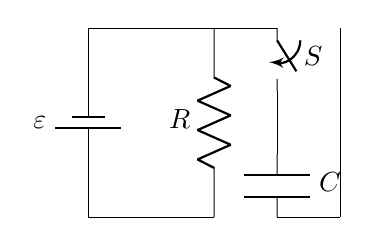
\begin{tikzpicture}[scale=0.8]
\draw (0,0) to[battery1, l=$\varepsilon$] (0,3);
\draw (0,3) -- (2,3);
\draw (0,0) -- (2,0);
\draw (2,0) to[resistor, l=$R$] (2,3);
\draw (4,0) -- (4,3);
\draw (2,3) -- (3,3);
\draw (3,0) -- (4,0);
\draw (3,3) to[switch, l=$S$] (3,2);
\draw (3,2) -- (3,1);
\draw (3,1) to[capacitor, l=$C$] (3,0);
\end{tikzpicture}
\caption{Kondansatörün şarj edildiği bir RC devresi}
\end{figure}

$t = 0$ anında anahtar kapatıldığında, kondansatör üzerinde henüz yük yoktur, bu nedenle $V_C(0) = 0$ olur. Başlangıçta akım maksimum değerdedir: $I(0) = \frac{\varepsilon}{R}$.

Kirchhoff Çevre Yasası'na göre:
\begin{align}
\varepsilon &= V_C + V_R\\
\varepsilon &= \frac{Q}{C} + IR
\end{align}

Zamana göre türev alındığında:
\begin{align}
0 &= \frac{1}{C}\frac{dQ}{dt} + R\frac{dI}{dt}\\
0 &= \frac{I}{C} + R\frac{dI}{dt}
\end{align}

Bu diferansiyel denklemin çözümü:
\begin{align}
\frac{dI}{I} &= -\frac{1}{RC}dt\\
\ln\frac{I}{I_0} &= -\frac{t}{RC}\\
I &= I_0 e^{-\frac{t}{RC}}\\
I &= \frac{\varepsilon}{R}e^{-\frac{t}{RC}}
\end{align}

Kondansatör üzerindeki gerilim:
\begin{align}
V_C &= \varepsilon - V_R\\
V_C &= \varepsilon - IR\\
V_C &= \varepsilon - \frac{\varepsilon}{R}Re^{-\frac{t}{RC}}\\
V_C &= \varepsilon(1 - e^{-\frac{t}{RC}})
\end{align}

Kondansatör üzerindeki yük:
\begin{align}
Q &= CV_C\\
Q &= C\varepsilon(1 - e^{-\frac{t}{RC}})
\end{align}

\begin{figure}[h]
\centering
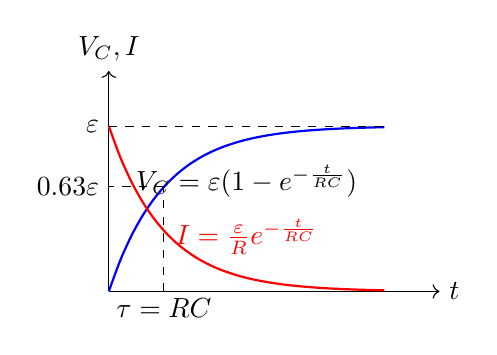
\begin{tikzpicture}[scale=0.7]
\draw[->] (0,0) -- (6,0) node[right] {$t$};
\draw[->] (0,0) -- (0,4) node[above] {$V_C, I$};
\draw (0,3) node[left] {$\varepsilon$};
\draw[domain=0:5, smooth, variable=\x, blue, thick] plot ({\x}, {3*(1-exp(-\x))});
\draw[domain=0:5, smooth, variable=\x, red, thick] plot ({\x}, {3*exp(-\x)});
\draw[dashed] (0,3) -- (5,3);
\draw[dashed] (1,0) -- (1,1.896);
\draw[dashed] (1,1.896) -- (0,1.896);
\draw (0,1.896) node[left] {$0.63\varepsilon$};
\draw (1,-0.3) node {$\tau = RC$};
\draw (2.5,2) node {$V_C = \varepsilon(1-e^{-\frac{t}{RC}})$};
\draw (2.5,1) node[red] {$I = \frac{\varepsilon}{R}e^{-\frac{t}{RC}}$};
\end{tikzpicture}
\caption{Kondansatör şarj sürecinde gerilim ve akımın zamana göre değişimi}
\end{figure}

\begin{tcolorbox}[title=SINAV İÇİN]
Şarj sürecinde $t = \tau = RC$ anında:
\begin{itemize}
\item $V_C = \varepsilon(1-e^{-1}) \approx 0.63\varepsilon$
\item $I = \frac{\varepsilon}{R}e^{-1} \approx 0.37\frac{\varepsilon}{R}$
\end{itemize}
\textbf{Pratik kural:} Bir kondansatör, $4\tau$ (4 zaman sabiti) sonra yaklaşık olarak tam şarj olmuş kabul edilir.
\end{tcolorbox}

\subsection{Kondansatörün Deşarj Edilmesi}

Şarj olmuş bir kondansatör bir direnç üzerinden deşarj edildiğinde, benzer şekilde eksponansiyel bir karakteristik gösterir.

\begin{figure}[h]
\centering
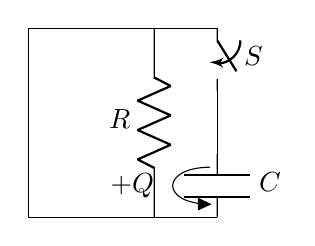
\begin{tikzpicture}[scale=0.8]
\draw (0,0) -- (0,3);
\draw (0,3) -- (2,3);
\draw (0,0) -- (2,0);
\draw (2,0) to[resistor, l=$R$] (2,3);
\draw (2,3) -- (3,3);
\draw (3,0) -- (2,0);
\draw (3,3) to[switch, l=$S$] (3,2);
\draw (3,2) -- (3,1);
\draw (3,1) to[capacitor, l=$C$, v=$+Q$] (3,0);
\end{tikzpicture}
\caption{Kondansatörün deşarj edildiği bir RC devresi}
\end{figure}

$t = 0$ anında anahtar kapatıldığında, kondansatör üzerindeki başlangıç gerilimi $V_C(0) = V_0$ olur.

Kirchhoff Çevre Yasası'na göre:
\begin{align}
0 &= V_C + V_R\\
\frac{Q}{C} &= -IR
\end{align}

Zamana göre türev alındığında:
\begin{align}
\frac{1}{C}\frac{dQ}{dt} &= -R\frac{dI}{dt}\\
\frac{I}{C} &= -RI
\end{align}

Bu diferansiyel denklemin çözümü:
\begin{align}
\frac{dQ}{Q} &= -\frac{1}{RC}dt\\
\ln\frac{Q}{Q_0} &= -\frac{t}{RC}\\
Q &= Q_0 e^{-\frac{t}{RC}}
\end{align}

Kondansatör üzerindeki gerilim:
\begin{align}
V_C &= \frac{Q}{C}\\
V_C &= \frac{Q_0}{C}e^{-\frac{t}{RC}}\\
V_C &= V_0 e^{-\frac{t}{RC}}
\end{align}

Devreden geçen akım:
\begin{align}
I &= \frac{dQ}{dt}\\
I &= \frac{d}{dt}(Q_0 e^{-\frac{t}{RC}})\\
I &= -\frac{Q_0}{RC}e^{-\frac{t}{RC}}\\
I &= -\frac{V_0}{R}e^{-\frac{t}{RC}}
\end{align}

\begin{figure}[h]
\centering
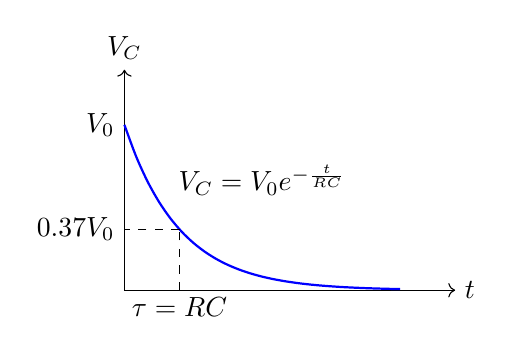
\begin{tikzpicture}[scale=0.7]
\draw[->] (0,0) -- (6,0) node[right] {$t$};
\draw[->] (0,0) -- (0,4) node[above] {$V_C$};
\draw (0,3) node[left] {$V_0$};
\draw[domain=0:5, smooth, variable=\x, blue, thick] plot ({\x}, {3*exp(-\x)});
\draw[dashed] (1,0) -- (1,1.104);
\draw[dashed] (1,1.104) -- (0,1.104);
\draw (0,1.104) node[left] {$0.37V_0$};
\draw (1,-0.3) node {$\tau = RC$};
\draw (2.5,2) node {$V_C = V_0 e^{-\frac{t}{RC}}$};
\end{tikzpicture}
\caption{Kondansatör deşarj sürecinde gerilimin zamana göre değişimi}
\end{figure}

\section{İndüktör (Bobin) İçeren DC Devreler}

\subsection{İndüktörün Akımlanması}

Bir indüktör DC kaynağa bağlandığında, akım yavaş yavaş artarak kararlı değerine ulaşır.

\begin{figure}[h]
\centering
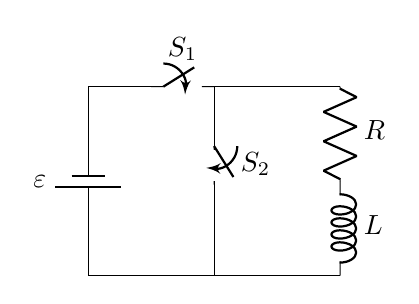
\begin{tikzpicture}[scale=0.8]
\draw (0,0) to[battery1, l=$\varepsilon$] (0,3);
\draw (0,3) -- (1,3);
\draw (0,0) -- (1,0);
\draw (1,3) to[switch, l=$S_1$] (2,3);
\draw (2,3) -- (4,3);
\draw (1,0) -- (4,0);
\draw (4,3) to[resistor, l=$R$] (4,1.5);
\draw (4,1.5) to[inductor, l=$L$] (4,0);
\draw (2,3) -- (2,2);
\draw (2,2) to[switch, l=$S_2$] (2,1.5);
\draw (2,1.5) -- (2,0);
\end{tikzpicture}
\caption{İndüktörün akımlandığı bir RL devresi}
\end{figure}

$S_1$ anahtarı kapatıldığında (ve $S_2$ açıkken), devreden akım geçmeye başlar. İndüktörün öz indüksiyonu, akımın aniden değişmesini engeller:
\begin{align}
\varepsilon_L = -L\frac{dI}{dt}
\end{align}

Kirchhoff Çevre Yasası'na göre:
\begin{align}
\varepsilon &= V_R + V_L\\
\varepsilon &= IR + L\frac{dI}{dt}
\end{align}

Bu diferansiyel denklemin çözümü:
\begin{align}
\frac{\varepsilon}{R} - I &= \frac{L}{R}\frac{dI}{dt}\\
\end{align}

Değişken değiştirerek ($x = \frac{\varepsilon}{R} - I$):
\begin{align}
x &= \frac{L}{R}\frac{dx}{dt}\\
\frac{dx}{x} &= -\frac{R}{L}dt\\
\ln\frac{x}{x_0} &= -\frac{R}{L}t\\
x &= x_0 e^{-\frac{R}{L}t}
\end{align}

Başlangıçta $t = 0$ anında $I = 0$ olduğundan, $x_0 = \frac{\varepsilon}{R}$ olur:
\begin{align}
\frac{\varepsilon}{R} - I &= \frac{\varepsilon}{R}e^{-\frac{R}{L}t}\\
I &= \frac{\varepsilon}{R}(1 - e^{-\frac{R}{L}t})
\end{align}

İndüktör üzerindeki gerilim:
\begin{align}
V_L &= L\frac{dI}{dt}\\
V_L &= L\frac{d}{dt}\left[\frac{\varepsilon}{R}(1 - e^{-\frac{R}{L}t})\right]\\
V_L &= \frac{\varepsilon L}{R}\frac{R}{L}e^{-\frac{R}{L}t}\\
V_L &= \varepsilon e^{-\frac{R}{L}t}
\end{align}

\begin{figure}[h]
\centering
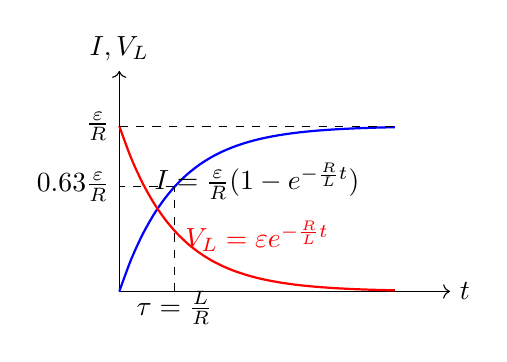
\begin{tikzpicture}[scale=0.7]
\draw[->] (0,0) -- (6,0) node[right] {$t$};
\draw[->] (0,0) -- (0,4) node[above] {$I, V_L$};
\draw (0,3) node[left] {$\frac{\varepsilon}{R}$};
\draw[domain=0:5, smooth, variable=\x, blue, thick] plot ({\x}, {3*(1-exp(-\x))});
\draw[domain=0:5, smooth, variable=\x, red, thick] plot ({\x}, {3*exp(-\x)});
\draw[dashed] (0,3) -- (5,3);
\draw[dashed] (1,0) -- (1,1.896);
\draw[dashed] (1,1.896) -- (0,1.896);
\draw (0,1.896) node[left] {$0.63\frac{\varepsilon}{R}$};
\draw (1,-0.3) node {$\tau = \frac{L}{R}$};
\draw (2.5,2) node {$I = \frac{\varepsilon}{R}(1-e^{-\frac{R}{L}t})$};
\draw (2.5,1) node[red] {$V_L = \varepsilon e^{-\frac{R}{L}t}$};
\end{tikzpicture}
\caption{İndüktör akımlanma sürecinde akım ve gerilimin zamana göre değişimi}
\end{figure}

\subsection{İndüktörün Deakımlanması}

$S_1$ anahtarı açılıp $S_2$ anahtarı kapatıldığında, indüktörde depolanan enerji direnç üzerinden boşalır.

Kirchhoff Çevre Yasası'na göre:
\begin{align}
0 &= V_R + V_L\\
0 &= IR + L\frac{dI}{dt}\\
L\frac{dI}{dt} &= -IR
\end{align}

Bu diferansiyel denklemin çözümü:
\begin{align}
\frac{dI}{I} &= -\frac{R}{L}dt\\
\ln\frac{I}{I_0} &= -\frac{R}{L}t\\
I &= I_0 e^{-\frac{R}{L}t}
\end{align}

Burada $I_0 = \frac{\varepsilon}{R}$ (indüktörün kararlı durum akımı):
\begin{align}
I &= \frac{\varepsilon}{R}e^{-\frac{R}{L}t}
\end{align}

\begin{tcolorbox}[title=SINAV İÇİN]
RL devrelerinde $t = \tau = \frac{L}{R}$ anında:
\begin{itemize}
\item Akımlanma: $I = \frac{\varepsilon}{R}(1-e^{-1}) \approx 0.63\frac{\varepsilon}{R}$
\item Deakımlanma: $I = \frac{\varepsilon}{R}e^{-1} \approx 0.37\frac{\varepsilon}{R}$
\end{itemize}
\textbf{Önemli:} Sınavda zaman sabitinin ne olduğunu açıklamanız istenebilir. $\tau = \frac{L}{R}$ ifadesini ve anlamını mutlaka belirtiniz.
\end{tcolorbox}

\section{Çözümlü Örnekler}

\subsection{Örnek 1: RC Devresi}

\begin{tcolorbox}
\textbf{Soru:} 250 V'luk bir DC güç kaynağı, 50 kΩ'luk bir direnç ve 0.001 μF'lık bir kondansatör içeren bir devrede, anahtar kapatıldıktan ne kadar zaman sonra kondansatör tam şarj olur? Ayrıca anahtar kapatıldıktan 100 mikro saniye sonra direncin iki ucu arasındaki potansiyel farkı nedir?
\end{tcolorbox}

\textbf{Çözüm:}
\begin{enumerate}
\item İlk olarak, zaman sabitini hesaplayalım:
\begin{align}
\tau = RC = 50 \times 10^3 \Omega \times 0.001 \times 10^{-6} \text{ F} = 50 \times 10^{-6} \text{ s} = 50 \text{ μs}
\end{align}

\item Kondansatörün tam şarj olması için pratik olarak $4\tau$ süresi gerekir:
\begin{align}
t_{\text{tam şarj}} = 4\tau = 4 \times 50 \text{ μs} = 200 \text{ μs}
\end{align}

\item Anahtar kapatıldıktan 100 μs sonra, direncin üzerindeki gerilim:
\begin{align}
V_R &= \varepsilon e^{-\frac{t}{RC}}\\
V_R &= 250 \text{ V} \times e^{-\frac{100 \times 10^{-6}}{50 \times 10^{-6}}}\\
V_R &= 250 \text{ V} \times e^{-2}\\
V_R &= 250 \text{ V} \times 0.135 = 33.7 \text{ V}
\end{align}

\item Kondansatör üzerindeki gerilim:
\begin{align}
V_C &= \varepsilon - V_R\\
V_C &= 250 \text{ V} - 33.7 \text{ V} = 216.3 \text{ V}
\end{align}
\end{enumerate}

\subsection{Örnek 2: RL Devresi}

\begin{tcolorbox}
\textbf{Soru:} 10 H'lik bir indüktör ve 100 Ω'luk bir direnç içeren bir devrede, anahtar kapatıldıktan sonra akımın maksimum değerinin \%63'üne ulaşması için geçen süre nedir? Ayrıca, yarı güç frekansını hesaplayınız.
\end{tcolorbox}

\textbf{Çözüm:}
\begin{enumerate}
\item Akımın maksimum değerinin \%63'üne ulaşması, bir zaman sabiti kadar sürede gerçekleşir:
\begin{align}
\tau = \frac{L}{R} = \frac{10 \text{ H}}{100 \text{ Ω}} = 0.1 \text{ s}
\end{align}

\item Yarı güç frekansı, indüktif reaktansın direnç değerine eşit olduğu frekanstır:
\begin{align}
\omega L &= R\\
2\pi f L &= R\\
f &= \frac{R}{2\pi L}\\
f &= \frac{100 \text{ Ω}}{2\pi \times 10 \text{ H}}\\
f &= \frac{100}{62.8} \text{ Hz} \approx 1.59 \text{ Hz}
\end{align}
\end{enumerate}

\begin{tcolorbox}[title=SINAV İÇİN MUHTEMEL SORULAR]
\begin{enumerate}
\item AC elektrik kaynağına bağlı 4.7 μF kondansatör ve 1.5 μF kondansatör, 650 H bobin ve 570 Ω dirençten oluşan bir devrenin eşdeğer direncini hesaplayınız.

\item Bir RC devresinde, anahtar kapatıldıktan ne kadar zaman sonra direncin uçlarındaki potansiyel belirli bir değere düşer?

\item RL devresinde, zaman sabitinin ne olduğunu açıklayınız ve bir devrede akımın maksimum değerinin \%99'una ulaşması için gerekli süreyi hesaplayınız.

\item AC kaynağa bağlı RC ve RL devrelerinin frekans cevabını çiziniz ve yarı güç frekansının önemini açıklayınız.
\end{enumerate}
\end{tcolorbox}



\section{Özet}

\begin{tcolorbox}
\textbf{RC Devreleri (Kondansatör içeren devreler):}
\begin{itemize}
\item Zaman sabiti: $\tau = RC$
\item Şarj durumunda kondansatör gerilimi: $V_C = \varepsilon(1 - e^{-\frac{t}{RC}})$
\item Şarj durumunda akım: $I = \frac{\varepsilon}{R}e^{-\frac{t}{RC}}$
\item Deşarj durumunda kondansatör gerilimi: $V_C = V_0 e^{-\frac{t}{RC}}$
\end{itemize}

\textbf{RL Devreleri (İndüktör içeren devreler):}
\begin{itemize}
\item Zaman sabiti: $\tau = \frac{L}{R}$
\item Akımlanma durumunda akım: $I = \frac{\varepsilon}{R}(1 - e^{-\frac{R}{L}t})$
\item Akımlanma durumunda indüktör gerilimi: $V_L = \varepsilon e^{-\frac{R}{L}t}$
\item Deakımlanma durumunda akım: $I = \frac{\varepsilon}{R}e^{-\frac{R}{L}t}$
\end{itemize}

\textbf{Pratik Kurallar:}
\begin{itemize}
\item Tam şarj/deşarj için gereken süre: $4\tau$
\item 1 zaman sabiti sonunda: \%63 şarj/akımlanma
\item 2 zaman sabiti sonunda: \%86 şarj/akımlanma
\item 3 zaman sabiti sonunda: \%95 şarj/akımlanma
\item 4 zaman sabiti sonunda: \%98 şarj/akımlanma
\end{itemize}
\end{tcolorbox}


\includegraphics[width=15cm]{Screenshot 2025-03-24 at 01-04-59 Claude.png}




\end{document}